\section{\textsc{Spring egg salad}}

\subsection*{Ingredients for 2 portions:}

\begin{tabular}{p{7.5cm} p{7.5cm}}
	& \\
	\textbf{For the salad:} & \textbf{For the sauce:} \\
	various leaf salads & 5tbsp fresh herbs \\
	1tbsp vinegar & 1 clove of garlic \\
	1tbsp olive oil & 1 shallot \\
	4 hard-boiled eggs & 1TL mustard \\
	salt und pepper & 3tbsp vinegar \\
	& 4tbsp olive oil
\end{tabular}

\subsection*{Serving suggestion:}

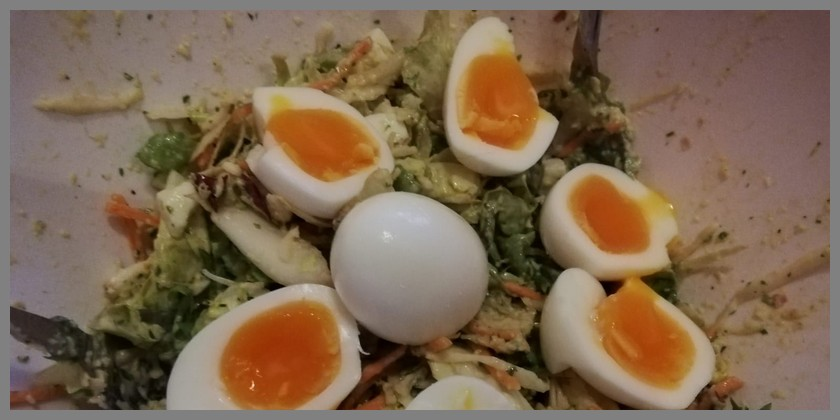
\includegraphics[width=\textwidth]{img/eiersalat.jpeg} \cite{fruehlingeiersalat}

\subsection*{How it's done:}

\begin{tabular}{p{15cm}}
	\\
  Cut the eggs in half and separate the egg yolk from the egg white. Peel and chop the garlic and shallots.\\
  Place the egg yolk, mustard, garlic and shallots in a measuring cup.\\
  Add the vinegar and oil and leave to stand for a few minutes.\\
  In the meantime, finely chop the herbs with a chopping knife. And add it to the other ingredients.\\
  Throw the egg whites in small cubes and add to the mixture.\\
  Puree finely and season to taste.\\
  Clean and chop the salads.\\
  Add oil, vinegar and spices and leave to stand for 10 minutes.\\
  Arrange in a large bowl and garnish with the remaining egg.\\
  Serve with 10 baguettes or fresh rolls.\\
  \textbf{Tip:}\\
  The salad makes itself super at Easter time. There are often boiled eggs left, which can be processed so well.
\end{tabular}
